\chapter{Introduction}\label{cha:intro}
What is given here is only meant to serve as a small introduction to some of the knowledge in physics which may be needed to understand this thesis.    
\newpage
\section{The main question in this thesis}
In this Bachelor's thesis the following question is of interest:\\
Does the inequality posed in the article \cite{PhysRevLett.101.020403} cover the real
part of the Bloch surface of a 3D quantum system when used as in~\cite{Kochen1968The}?\\
This will be done by evaluating the Klyachko inequality with the measurements produced by Kochen and Specker and then plotting this onto the Bloch sphere.
To understand the questions and how this will be done, some introduction is needed.\\
This topic was chosen in collaboration with my mentor for its interesting applications and also my interest in the field of contextuality. An interesting thing to note, in this field most discussion has been applied to spin 1/2 systems, and not any other system.
\section{Background of quantum mechanics}\label{sec:intro:Background of quantum mechanics}
Most of this section can be found in any university course in quantum mechanics. The material for this chapter has been based on the course given at Linköpings University with~\cite{Bransden:2000}
as the course literature. For more details consult the book. 
\subsection{The origin of quantum mechanics}
In the beginning of the 20th century, some physical phenomena could not be explained by classical physics, for example the ultra-violet disaster of any classical model of of black-body radiation, and the photoelectric effect. There were many other phenomena that were unexplainable, for more see for instance~\cite{Bransden:2000}.
It was these phenomena that led to the formulation of quantum mechanics, where energy transfer is quantized and particles can act as both waves and particles at the same time. Another big distinction between classical physics and quantum mechanics is that now it is more common to speak of statistical measurements, this is why quantum mechanics can be seen as an extension of statistical mechanics.
Statistical data such as the average value and the standard deviation is used to draw conclusions and compare several performed measurements on a system. A common operation in quantum mechanics is to take the statistical average known as the expectation value for a system.    

The most famous and by most considered the basic equation of quantum mechanics was discovered when E.\ Schrödinger was exploring the physics of small particles. A full derivation of this can be found in the original paper,~\cite{Schrodinger:1926}, or in a course of Analytical Mechanics. What he arrived at is known as the Schrödinger equation, with $\vec{x}$ as the position and t as the time, 
\begin{equation} \label{eq:Schrödinger}
i\hbar\frac{\partial}{\partial t}\psi (\vec{x}, t) = \hat{H}\psi (\vec{x}, t)
\end{equation}
which can be interpreted in the following way:
Since both i and $\hbar$ are constants, one can basically say that the time derivative of the wave-function is equal to the Hamiltonian of system acting on the wave-function. The Hamiltonian will not be discussed here, however it is a concept that is discussed a lot in the field of Analytical Mechanics.
It is the wave-function of a system that has the most interest in quantum mechanics. 
Not to forget, another important property of quantum mechanics is that nothing can be known about a system until it has been measured. It was this that was explained through the Schrödinger cat thought experiment. See more in the translation of the original paper ~\cite{Schrodinger:1980}.

Many new properties have been discovered through quantum mechanics, for instance that elementary particles and atoms have spin. Some more details can be found by studying classical angular momentum and how it continues in quantum mechanics. It is through this that the mathematics for spin is deduced. This will be discussed further in~\ref{sec:intro:Background of quantum mechanics:Finite dimentional quantum-states}
\subsection{Dirac bra-ket notation}\label{subsec:Dirac bra-ket notation}
By solving the Schrödinger equation, see equation (\ref{eq:Schrödinger}), a wave-function for a system can be found and utilized for calculations. From here on the wave-function will be denoted as a state: $|\psi\rangle$.
Here also the dependent variables are omitted for simplicity such that:
$$|\psi\rangle = \psi (\vec{x}, t)$$
This notation is known as the Dirac bra-ket notation, where the above is known as a ket-vector. Throughout this thesis the use of the word state and vector can be considered to be equal, since the state is represented as a vector in Hilbert space, see more in a course in functional analysis or~\cite{Kreyzig}. The bra-ket notation comes with certain notations, such as: $|\psi\rangle^\dagger = \langle\psi|$, the latter known as a bra-vector. Where $\dagger$ denotes the complex-conjugate. $\langle\psi|\psi\rangle =$ modulus of the vector $\psi$\\
Only a few details have been mentioned here. Using the bra-ket notation,~\ref{eq:Schrödinger} can be rewritten as: \begin{equation} \label{eq:Schrödinger2}
i\hbar\frac{\partial}{\partial t}|\psi\rangle = \hat{H}|\psi\rangle
\end{equation}
\subsection{Operator formalism}\label{sec:intro:Background of quantum mechanics:Operator formalism}
An observable corresponds to a value which can be measured, such as position, momentum, energy etc. Also, to be remembered from above, that in most cases, and in this thesis, conclusions can only be made from the expectation values of the observables. To note, there can be observables that can only be true or false. What is actually done is calculating the eigenvalues for the operators in Hilbert space. In the quantum mechanical framework, one utilizes so called operators to produce different observables. An example of this is the operator $\hat{x} = i\hbar\frac{\partial}{\partial p}$   
which when used or applied to a state will produce the position of the state.  So, mathematically to calculate the position would look something like this: $\langle\psi|\hat{x}|\psi\rangle$ 
\subsection{Commutating operators}
What does commutation mean?
Putting it simply, is is the ability to let two operators act after each other without the first one changing the result for the other. As an example: $\langle\psi|\hat{A}\hat{B}|\psi\rangle$ should produce the same value as $\langle\psi|\hat{B}\hat{A}|\psi\rangle$ if $\hat{A}$ and $\hat{B}$ commute. Subtracting these both should then equal zero. This is usually written as $[\hat{A},\hat{B}]$ where, to be evaluated should act on a state.
Some operators commute and some do not. A famous example of this is that the operator for momentum and position do not commute. So it is not possible to know the position and momentum of a state, for instance a particle, at the same time. It is from this one gets the Heisenberg uncertainty, see more details in~\cite{Bransden:2000}.

This is all a continuation of the fact that a measurement of a quantum-state will collapse the state, meaning that once a measurement has been done to the state, the simultaneous measurement of the second operator can not be accurately performed. Thus, the standard deviation increases dramatically when trying to measure two non-commuting operators. It is thus said that measuring one observable will destroy all simultaneous measurements for non commuting observables.
\subsection{Finite dimentional quantum-states}\label{sec:intro:Background of quantum mechanics:Finite dimentional quantum-states}
The most useful and known states are the spin 1/2 systems. It is this state which is used for one implementation for qubits used in quantum computing. This is also how the free electron spins. 

For the free electron one can show that the quantum-state must be in the following form: $$|\psi\rangle=a_0|+\frac{1}{2}\rangle+a_1|-\frac{1}{2}\rangle$$ which can be explained as a superposition between spin up and spin down.
By letting the ket-vector be normalized, meaning that $|a_0|^2+|a_1|^2=1$, the measurements can be interpreted as statistical. This means that measuring the spin will result in spin up with probability $|a_0|^2$ and $|a_1|^2$ for spin down.  In this article only systems with spin one and composed of one particle are discussed. This means that the state can be written as: $$|\psi\rangle=a_0|-1\rangle+a_1|0\rangle+a_2|1\rangle$$ where the coefficients should still be normalized. 
\subsection{Bloch Sphere}\label{Bloch Sphere}
There can be an infinite set of quantum-states that will explain the spin of a free electron. How can this be visualized in an easy way? Staying with spin 1/2 to start off. Using the normalization condition of the bra-vector from above, $|a_0|^2+|a_1|^2=1$, and some elementary mathematics the vector can be rewritten as:
$$|\psi\rangle=e^{i\gamma}(\cos(\frac{\theta}{2})|+\frac{1}{2}\rangle+e^{i\phi}\sin(\frac{\theta}{2})|+\frac{1}{2}\rangle)$$
Since the measurement will not be affected by the first factor, since the modulus squared of $e^{i\gamma}$ is equal to 1, this means that the state can be written as:
$$|\psi\rangle=\cos(\frac{\theta}{2})|+\frac{1}{2}\rangle+e^{i\phi}\sin(\frac{\theta}{2})|+\frac{1}{2}\rangle$$
Visualizing a vector with modulus 1 and two angles will produce a unit-sphere. See figure~\ref{fig:Bloch}, where the spins are written now as 0 or 1 and the axis are chosen simply for artistic reasons. More of this can be seen in~\cite{Nielsen:2010}.
\begin{figure}[h]
\begin{center}
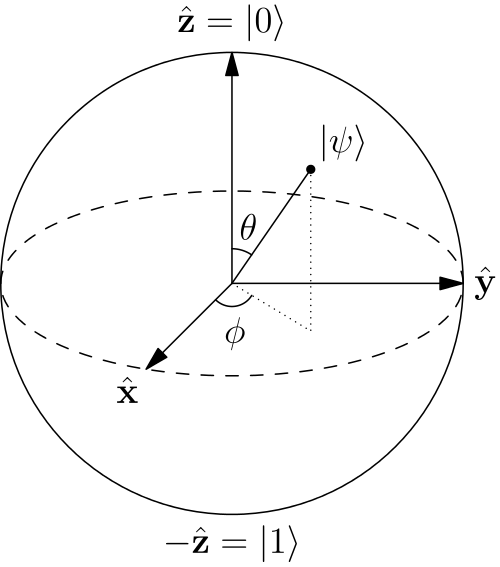
\includegraphics[scale=0.2]{Bloch_Sphere.png} 
\caption{Bloch sphere}
\label{fig:Bloch}
\end{center}
\end{figure}
Going over to a spin 1 system, there is a slight problem. Since the coefficients can be complex, there would need to be in total 6-axis for the visualisation, which is more than the 3 that can be visualized by us. To solve this conundrum, let the coefficients be real. By letting each of the axis represent one of the spins, i.e taking $\hat{x}=|-1\rangle, \hat{y}=|0\rangle, \hat{z}=|1\rangle$ the visualization can be done in the same way as before for the spin 1/2 system. 
\newpage
\section{Non-contextuality inequalities}\label{sec:intro:Noncontextuality inequalities}
\subsection{What is contextuality?}\label{sec:intro:Background of quantum mechanics:What is contextuality?}
Contextuality refers to when the result of an experiment depends on the context of the experiment. In quantum mechanics an example of this would be when measuring two observables, their measurements will depend on each other even though they commute. This means that the set-up of the system will influence the outcome of the measurements.
The opposite of this is of course non-contextuality where the commuting property is not dependent on the experiment.
An interesting special case of non-contextuality is known as locality. Locality states that there can be no interaction at a distance. Here distance only means that nothing can influence outside of it's light cone, which means that locality ensures causality and forbids information to travel faster than the speed of light in vacuum.
\subsection{How do we get the contextual inequalities?}
Simply put, one finds a condition which if fulfilled shows that there is a non-contextual hidden variable schema. If the condition is violated, then there is no non-contextual hidden variable schema.\\
To note, the hidden variable schema is another schema for explaining quantum mechanical phenomena. The inequalities are found through the hidden variable schema which means that they might not hold for a quantum mechanical schema. The interesting case is where the inequality is violated in a quantum mechanical description.\\
Below a few inequalities are explained.
\subsection{The CHSH inequality}\label{sec:intro:Background of quantum mechanics:The CHSH inequality}
CHSH stands for John Clauser, Michael Horne, Abner Shimony and Richard Holt who described the inequality in the article~\cite{PhysRevLett.23.880}, see it here below.
\begin{equation*}
\langle A_1 A_2 \rangle + \langle A_2 A_3 \rangle + \langle A_3 A_4 \rangle - \langle A_4 A_1 \rangle \leq 2
\end{equation*}
The inequality was found through a proposed experiment that would test the hidden variable schemas. Though eventually, the inequality states the same as Bell's inequality. 

Bell's inequality is based on a system where two electrons have been prepared so that they, when measured together must always have a total spin value of 0.
If there is nothing to influence the measurement to either of the spins, we can write the states with equal probability as: $|\psi\rangle = \frac{|+-\rangle + |-+\rangle}{\sqrt{2}}$
This is a so called bell state, an entangled state as discussed above.
By measuring one of the electrons spin, it is then know that the other electron must have opposite spin, since the total spin must be fixed, here at 0. If the conditions are met it is called a Bell state.

Using the Bell state, a thought experiment was proposed by EPR, Einstein, Podolsky and Rosen. In this experiment, the electrons have been separated a distance, it need not be big, however there must be a distance. What is then proposed is that a measurement is done on the first electron. Through the fixed spin, the spin of the second electron is known. This seems to suggest that information has travelled the distance between the electrons in an instance. Making the distance big enough would then violate special relativity. Another interesting problem is that a measurement of the first electron will not collapse the second electrons state. Meaning that one could measure position of the first and momentum of the second electron and then through logic violate the non-commuting property of these observables.
Something must be wrong above, either there is some inherit property in the electrons that "knows" what value it must have so that information is not sent. This is usually called a hidden variable schema and more can be seen in the article by~\cite{PhysRev.47.777}.

After this paper was written, the theorem of hidden variables was disproved in the paper by ~\cite{Bell:1964}, this was done by showing that the schema of local hidden variables can not reproduce all consequences of quantum entanglement. A note of interest to the rest of the thesis. The deduction of this inequality has only used two spin 1/2 systems, whereas this thesis will discuss spin 1 systems.
\subsection{Kochen–Specker theorem}
Another interesting theorem used for quantum-mechanical contextuality is the Kochen-Specker theorem, which can be seen as a complement to Bell's theorem. This is since they describe the same concept, but in this case for spin 1 particles instead of spin 1/2 particles. In this sense Bell's theorem is much simpler. For all the details see the original paper~\cite{Kochen1968The}. Interestingly enough, this paper was published before the CHSH paper, though all details were first understood after they were both published.
The theorem proves that quantum-mechanics can not be described by a hidden variable schema,thus observables always have definite values and that the observables are non-contextual.

This is done by identifying a set of finite 1-dimensional projection operators in a 3-dimensional Hilbert space, in which a projection operator can belong to different orthogonal triplets of projection operators. These in turn represent different measurement contexts. This means that no assignment of the value 0 or 1 is possible to any of the projection operators while still in non-contextuality and respecting the orthogonality relation. The latter comes from that a if a projection operator has the value 1 then any orthogonal projection operator must be assigned the value 0. A very good introduction can be found in \cite{Bub2010}

This means that the assumptions made by EPR have been proven to be impossible since now a hidden variable schema must be contextual. This theorem is even stronger than the one given by Bell, since the later is only related to locality which is a subset of non-contextuality. 
Because of this theorem it is now known that a schema including hidden variables must contextual.
What should be taken from this paper are the following:\\
\cite{Kochen1968The} show mathematically that depending on how you define your measurements directions you will get different results, thus contextuality. Through this 117 measurement vectors can be produced and it is these that will be used in the thesis. 
\subsection{The inequality}\label{sec:intro:Background of quantum mechanics:Ine}
In the article by~\cite{PhysRevLett.101.020403}, the following inequality is given:
\begin{equation} \label{eq:Inequality}
\langle A_1 A_2 \rangle + \langle A_2 A_3 \rangle + \langle A_3 A_4 \rangle + \langle A_4 A_5 \rangle +
\langle A_5 A_1 \rangle \geq -3
\end{equation}
This inequality, known as the pentagram inequality, which can be formulated into the CHSH inequality by choosing $A_5 = -A_1$.
In the same way as the CHSH inequality, if a violation is found for a state, then it has been shown that the state has a nonclassical behaviour. The pentagram inequality is valid for only non-contextual hidden variables, as is the CHSH inequality. Before this is proven, the interesting clash between this and the Kochen-Specker theorem must be addressed.

In the subsection above it was stated that a hidden variable schema must be contextual. The pentagram inequality is valid for non-contextual hidden variables but is violated by quantum mechanics. This, and the reason that it is much easier to test is why this is used in the rest of the thesis to prove Kochen-Specker.

How is it now seen that the inequality in not valid for contextual hidden variables, contrary to what is stated in the paper~\cite{PhysRevLett.101.020403}. In the hidden variable schema our $A_i$ can only be chosen as integers, $A_i = 1, -1$ through context they are chosen so that each $\langle A_iA_j \rangle = -1$. This means that the inequality will have the value $-5$ which is not greater or equal to $-3$. Through this simple choice no rules are violated, though the inequality is. \\
For non-contextuality, the choice is definite, not depending on the brackets. Meaning that choosing values  -1 and 1 for all $A_i$ will never violate the inequality. In quantum mechanics the values are not directly known. Before starting the next section, it is known that inequality should not hold for quantum mechanical description since it is derived from the hidden variable schema.
\\
In the next section the projection operators will be used, and several states/vectors tested.